\documentclass[11pt,a4paper]{article}

\usepackage[utf8]{inputenc}
\usepackage[T1]{fontenc}
\usepackage{amsmath,amssymb}
\usepackage{graphicx}
\usepackage{booktabs}
\usepackage{xcolor}
\usepackage[margin=1.1in]{geometry}
\usepackage[colorlinks=true,linkcolor=blue!60!black,citecolor=blue!60!black,urlcolor=blue!60!black]{hyperref}

\newcommand{\Gstar}{{G^{*}}}
\graphicspath{{figures/}}

\title{\bfseries The Clock at the Edge of Stability}
\author{C.~Pacitani\thanks{Draft v2, 2026-08-05 (v1 audited refute-by-default;
corrections applied). Interactive companion and all simulation/analysis code
accompany this manuscript. Section~\ref{sec:data} is reserved for measured
data; all quantitative results herein are exact theory or simulation.}}
\date{}

\begin{document}
\maketitle

\begin{abstract}
Galileo founded timekeeping on isochronism: a harmonic clock's period ignores
its amplitude, and the constant governing it is $\pi$. Exactly at a symmetric
instability threshold --- a column at critical load, a mode at a pitchfork
bifurcation --- the quadratic restoring term vanishes and the generic surviving
dynamics is the \emph{pure quartic} oscillator, whose behavior is the
anti-pendulum: its frequency is proportional to its own amplitude. Its period
constant is not $\pi$ but $\Gstar=\Gamma(\tfrac14)/\Gamma(\tfrac34)=
2.9586751\ldots$, the lemniscate's analogue of the circle constant. We present
this ``clock of marginal stability'' as a self-contained piece of classical
physics: the threshold normal form, the exact period law
$T=\sqrt{\pi}\,\Gstar\sqrt{m/2\lambda}/A$, its elliptic generalization off the
edge, and a battery of calibration-free signatures --- the linear
frequency--amplitude law, a dimensionless waveform functional
$\mathcal B_4=48\pi/\Gstar^{4}$, and quantum level scaling
$E_n\propto n^{4/3}$. A two-spring tabletop realization makes the potential
purely quartic \emph{by symmetry} rather than by tuning, and end-to-end
simulations of that apparatus, including its dominant systematics, recover
$\Gstar$ to $0.3\%$ with no fitted scale. An interactive in-browser laboratory
accompanies the paper.
\end{abstract}

\section{The anti-pendulum}
\label{sec:intro}

Every introductory course teaches one clock. The harmonic oscillator's period
$T=2\pi\sqrt{m/k}$ is independent of amplitude, and that isochronism ---
noticed by Galileo for small swings, and engineered into exactness by Huygens,
who knew the circular pendulum's isochronism is only approximate and built the
cycloidal pendulum to repair it \cite{huygens} --- is why pendulums, balance
wheels, and $LC$ circuits keep time. The constant that converts the system
scales into a duration is $\pi$: the circle constant, because the phase-space
orbit of a harmonic oscillator is an ellipse traversed uniformly.

This paper is about the complementary clock, the one that lives where the
harmonic term \emph{vanishes}. Its restoring force is $F=-4\lambda x^{3}$, its
potential the flat-bottomed quartic $V=\lambda x^{4}$, and its period is
\begin{equation}
\boxed{\;T \;=\; \sqrt{\pi}\;\Gstar\,\sqrt{\frac{m}{2\lambda}}\;\frac{1}{A}\;,
\qquad
\Gstar \;=\; \frac{\Gamma(\tfrac14)}{\Gamma(\tfrac34)} \;=\; 2.958675119188639\ldots}
\label{eq:period}
\end{equation}
where $A$ is the turning-point amplitude. Two features deserve immediate
emphasis. First, the period \emph{depends on amplitude} --- frequency grows
linearly with $A$. This clock counts how hard it swings; it is the
anti-pendulum. Second, the role of $\pi$ has been taken over by a different
classical constant, $\Gstar$, which is to the \emph{lemniscate} what $\pi$ is
to the circle: writing $\varpi=2.622057\ldots$ for the lemniscate constant
(half the arc length of the unit lemniscate $r^{2}=\cos2\theta$), one has
$\Gstar = 2\varpi/\sqrt{\pi}$, so that $\sqrt{\pi}\,\Gstar$ \emph{is} the
total arc length of the unit lemniscate, precisely as $2\pi$ is the
circumference of the unit circle. The solution of the quartic oscillator is
the lemniscatic sine of Gauss and Abel, as the harmonic solution is the
circular sine; the mathematics descends directly from Fagnano's
eighteenth-century division of the lemniscatic arc and Gauss's
arithmetic--geometric mean \cite{ww,siegel}.

Why should a physicist care about a clock nobody builds on purpose? Because
nature builds it at every \emph{symmetric instability threshold}, and
thresholds are everywhere.

\section{The threshold theorem}
\label{sec:threshold}

Consider any one-degree-of-freedom system with a reflection symmetry
$x\to-x$, smoothly tuned by a parameter $\mu$ through a symmetric (pitchfork)
instability at $\mu=0$:
\begin{equation}
V(x;\mu) \;=\; \tfrac12\,\mu\,x^{2} \;+\; \lambda\,x^{4} \;+\; O(x^{6}),
\qquad \lambda>0 .
\label{eq:normalform}
\end{equation}
For $\mu>0$ the well is harmonic; for $\mu<0$ it splits into a double well.
\emph{Exactly at threshold} the quadratic term is gone and the generic leading
behavior --- generic because the cubic is forbidden by symmetry, not by
tuning --- is the pure quartic. Equation~\eqref{eq:normalform} is the normal
form of a perfect Euler column at critical load (a supercritical, or
stable-symmetric, buckling instability), of any order parameter at a
continuous symmetry-breaking transition treated at mean-field level
\cite{landau}. The quartic oscillator is therefore not an exotic special
case: it is \emph{the universal clock of marginal stability}, the timekeeping
that remains when a mode has gone soft symmetrically.

The full period law across the threshold follows from one quadrature. With
turning point $A$ and energy $E=\tfrac12\mu A^{2}+\lambda A^{4}$,
\begin{equation}
T(A;\mu)
\;=\;
4\sqrt{\frac{m}{2}}\;
\frac{K(\kappa)}{\sqrt{\tfrac{\mu}{2}+2\lambda A^{2}}},
\qquad
\kappa^{2} \;=\; \frac{\lambda A^{2}}{\tfrac{\mu}{2}+2\lambda A^{2}},
\label{eq:elliptic}
\end{equation}
where $K$ is the complete elliptic integral of the first kind (modulus
convention). The two limits close exactly: at $\mu=0$,
$\kappa^{2}=\tfrac12$ and $K(1/\sqrt2)=\Gamma(\tfrac14)^{2}/4\sqrt{\pi}$
reproduce Eq.~\eqref{eq:period}; at $\lambda=0$, $K(0)=\pi/2$ gives
$2\pi\sqrt{m/\mu}$. The value $\kappa=1/\sqrt2$ is the \emph{self-dual
modulus} --- the fixed point of the exchange $k\leftrightarrow k'$ between a
modulus and its complement, where $K'=K$ --- and it is where every appearance
of $\Gstar$ in classical analysis originates; the reader may recognize it
from the $90^\circ$ pendulum, whose exact period is
$4\sqrt{L/g}\,K(1/\sqrt2)$.

Equation~\eqref{eq:elliptic} also supplies the experimental narrative
(Fig.~\ref{fig:edge}b): at small amplitude a residual $\mu$ dominates and the
period saturates at the harmonic value; at large amplitude every curve joins
the universal $T\propto1/A$ quartic branch; the crossover amplitude measures
the distance to the edge. Tuning $\mu\to0$ pushes the harmonic plateau out of
the observable window --- the signature that one has arrived at the edge is
that \emph{the clock forgets how to be isochronous at all amplitudes}.

\begin{figure}[t]
\centering
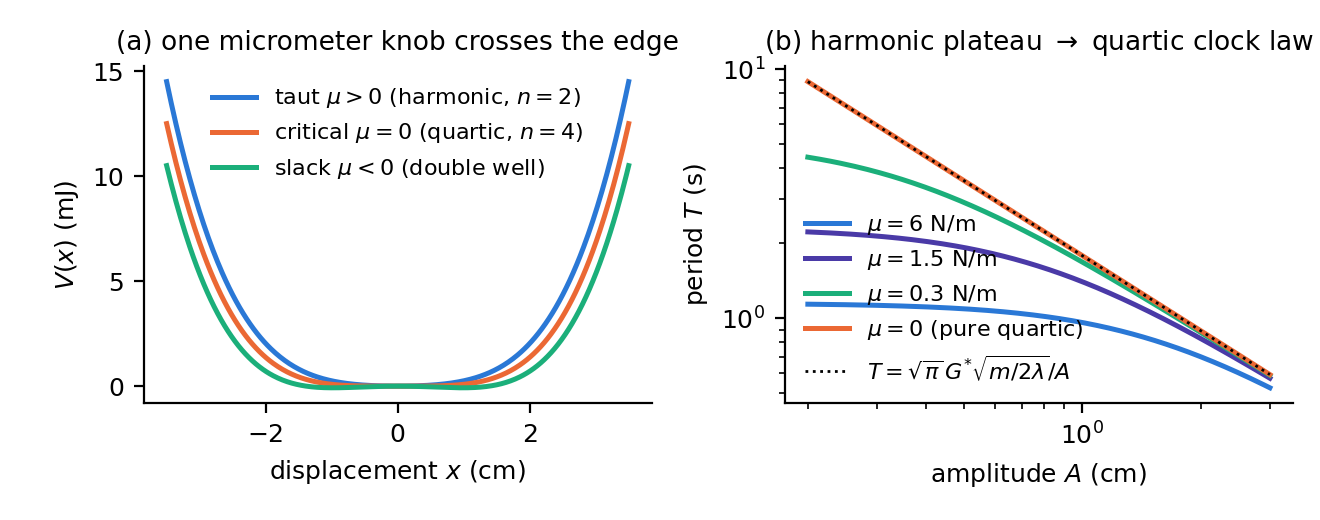
\includegraphics[width=\textwidth]{fig1_edge.pdf}
\caption{(a) The two-spring potential of Sec.~\ref{sec:apparatus} at three
micrometer settings: taut ($\mu>0$, harmonic), critical ($\mu=0$, pure
quartic), slack ($\mu<0$, double well). One knob traverses the pitchfork.
(b) The period law Eq.~\eqref{eq:elliptic}: harmonic plateaus at small
amplitude joining the universal quartic branch $T=\sqrt{\pi}\,\Gstar
\sqrt{m/2\lambda}/A$ (dotted).}
\label{fig:edge}
\end{figure}

\section{Calibration-free signatures}
\label{sec:signatures}

The quartic clock offers unusually clean tests because its key signatures are
dimensionless or scale-free.

\paragraph{S1 --- the clock law.} On the quartic branch $T\cdot A$ is constant
and
\begin{equation}
\Gstar_{\mathrm{exp}} \;=\; T\,A\,\sqrt{\frac{2\lambda}{\pi m}}
\label{eq:recovery}
\end{equation}
recovers the lemniscatic constant with \emph{no fitted scale}: $\lambda$ comes
from a static force--displacement measurement, $m$ from a scale. In log--log
form the signature is a frequency--amplitude slope of exactly $+1$
(a harmonic clock gives $0$).

\paragraph{S2 --- the waveform functional.} The pure-quartic waveform is the
lemniscatic sine, visibly flatter-topped than a sinusoid. Parameterizing one
cycle by uniform phase $\theta\in[0,2\pi)$ and writing
$x'=dx/d\theta$, the ratio
\begin{equation}
\mathcal B \;=\; \frac{2\,\langle x^{2}\rangle}{\langle x'^{2}\rangle}
\label{eq:B}
\end{equation}
is invariant under changes of amplitude, of time unit, and of overall scale.
For the potential family $V\propto |x|^{p}$ one finds
$\mathcal B_2 = 2$ exactly (sinusoid), while the quartic member evaluates to
\begin{equation}
\mathcal B_4 \;=\; \frac{48\pi}{\Gstar^{4}} \;=\; 1.9678953151\ldots,
\qquad
\mathcal B_6 \;=\; \frac{24\pi^{3}}{B(\tfrac16,\tfrac12)^{3}}
= 1.9239861993\ldots
\label{eq:B4}
\end{equation}
(with $B$ the Euler beta function); the derivation is two lines from the
virial moment $\langle x^{2}\rangle = 4/\Gstar^{2}$ and the phase-speed
identity $\langle x'^{2}\rangle = \Gstar^{2}/6\pi$ of the normalized quartic
waveform. The $1.6\%$ depression of $\mathcal B$ below $2$ is a pure number:
measuring it requires no calibration of anything.

\paragraph{S3 --- quantum level scaling.} The phase-space area at energy $E$
is $J(E) = \tfrac{2}{3}\,\Gstar\sqrt{2\pi m}\;\lambda^{-1/4}E^{3/4}$, so
Bohr--Sommerfeld quantization gives $E_n \propto n^{4/3}$ --- against the
harmonic $E_n\propto n$. Anharmonic superconducting circuits tuned to a
quartic point \cite{quarton}, or particles in quartic optical traps, would
realize this rung.

\section{A tabletop realization that is quartic by symmetry}
\label{sec:apparatus}

The experimental difficulty at any critical point is staying there:
imperfections detune $\mu$ away from zero. The following geometry sidesteps
half of the problem by making the \emph{odd} terms vanish identically rather
than approximately. A mass $m$ sits midway between two anchors separated by
$2L$, held by two identical springs (stiffness $k$, natural length $L_0$).
For transverse displacement $x$ each spring has length $\sqrt{L^{2}+x^{2}}$;
with the springs exactly at natural length ($L=L_0$) the extension is
second order in $x$, and the total potential is
\begin{equation}
V(x) \;=\; \frac{k}{4L^{2}}\,x^{4}\;+\;O(x^{6}),
\qquad \lambda = \frac{k}{4L^{2}},
\label{eq:springquartic}
\end{equation}
with the reflection symmetry exact by construction --- no cubic term is
possible, tuned or not. Pretension $\delta=L-L_0$ reintroduces
$\mu = 2k\delta/L$, so a single micrometer on one anchor walks the system
through the full pitchfork of Fig.~\ref{fig:edge}a. At a representative
design point ($k=500$\,N/m, $L=12$\,cm, $m=200$\,g) the periods in the
working amplitude window of $1.0$--$2.4$\,cm run from $0.74$ to $1.78$\,s in
the $\mu=0$ idealization (from $0.72$ to $1.42$\,s once the suspension term
of Sec.~\ref{sec:validation} is included) --- comfortable territory for
camera tracking.

Because the frequency tracks its own amplitude, a \emph{single ringdown
sweeps the entire} $T(A)$ \emph{curve}: per-cycle periods from successive
zero crossings, per-cycle amplitudes from the geometric mean of bracketing
peaks. Ten ringdowns constitute a complete dataset for
Eq.~\eqref{eq:recovery}.

\begin{figure}[t]
\centering
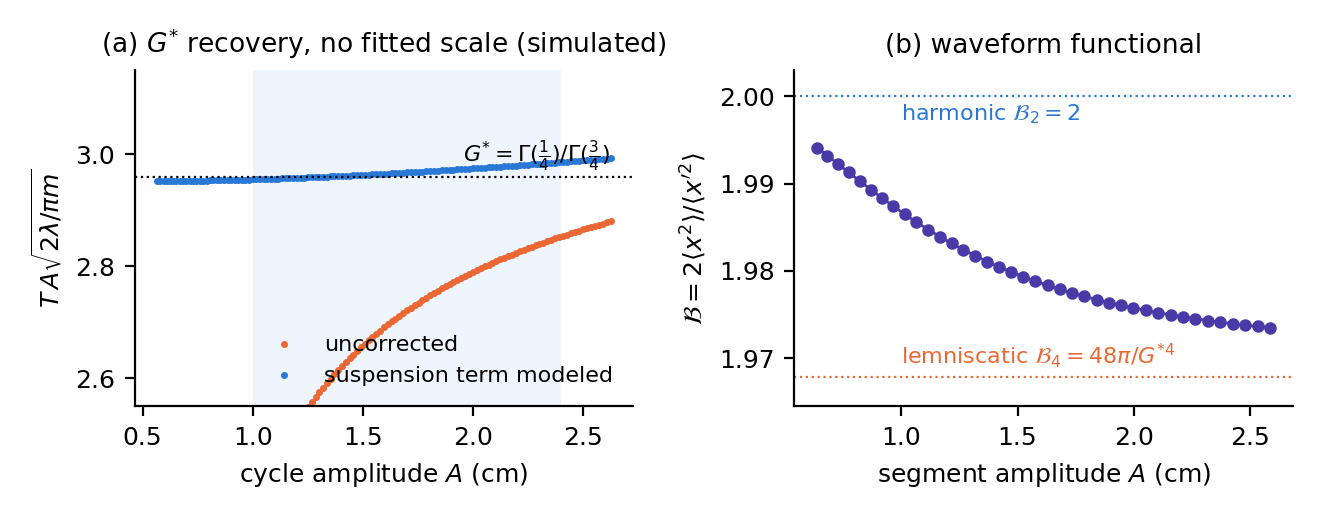
\includegraphics[width=\textwidth]{fig2_recovery.pdf}
\caption{End-to-end \emph{simulation} of the apparatus of
Sec.~\ref{sec:apparatus}, including the exact (untruncated) spring geometry,
the suspension's gravitational restoring term, and damping ($Q\approx300$).
(a) The calibration-free combination $T\,A\sqrt{2\lambda/\pi m}$ per cycle:
ignoring the suspension term biases the recovery ($-8\%$, orange); modeling
it with Eq.~\eqref{eq:elliptic}, with $\mu$ pinned at its known value
(experimentally: by an independent pendulum-period measurement), recovers
$\Gstar$ to $+0.28\%$ (blue; shaded band = declared analysis window).
(b) The waveform functional Eq.~\eqref{eq:B}, extracted with per-cycle phase
mapping, descending from near the harmonic value $2$ toward the lemniscatic
$\mathcal B_4$ as amplitude grows into the quartic branch.}
\label{fig:recovery}
\end{figure}

\section{Simulated validation and error budget}
\label{sec:validation}

Before any hardware, the full measurement chain was validated against a
synthetic apparatus that includes what the idealization omits: the exact
two-spring geometry (whose $x^{6}$ softening shifts the period by $+0.3\%$ at
$A=0.1L$ and $+1.2\%$ at $A=0.2L$, setting the window edge), a
bifilar-suspension gravitational term $\mu_g = mg/\ell$ (which is \emph{not}
small --- at $\ell=1.5$\,m it shifts small-amplitude periods by up to
$\sim25\%$ and must be modeled, not ignored), and linear damping. The
declared analysis --- Eq.~\eqref{eq:elliptic} with $\mu$ pinned at its
independently known value --- recovers (Fig.~\ref{fig:recovery}a) a
frequency--amplitude slope of $0.988$ and $\Gstar$ to $+0.28\%$, robust to a
deliberate $\pm5\%$ mis-pin of $\mu$ ($+0.70\%/-0.12\%$). The residual bias
is the booked $x^{6}$ term. The waveform functional
(Fig.~\ref{fig:recovery}b) requires one procedural rule discovered in
simulation: because this clock chirps, each cycle must be mapped onto its own
$2\pi$ of phase before averaging --- resampling several cycles against a
single fixed period smears phase and spuriously pushes $\mathcal B$
\emph{above} $2$. With per-cycle mapping the extractor is unbiased at the
$3\times10^{-5}$ level on exact controls, and the simulated ringdown
traverses $\mathcal B = 1.994\to1.974$, descending from near the harmonic
value toward $\mathcal B_4$ as amplitude grows into the quartic branch.

The projected error budget for $\Gstar_{\mathrm{exp}}$ --- static $\lambda$
calibration ($1\%$), effective mass ($0.8\%$), amplitude calibration
($0.5\%$), residual-$\mu$ modeling ($0.5\%$), geometric $x^{6}$ ($0.5\%$) ---
combines, through the square roots in Eq.~\eqref{eq:recovery}, to
$\approx1.1\%$.

\section{Measured data}
\label{sec:data}

\emph{[Reserved. This section will report the ringdown datasets, the
$T(A;\mu)$ global fit across micrometer settings, the recovered
$\Gstar_{\mathrm{exp}}$ with its uncertainty, and the measured
$\mathcal B(A)$ trend, against the gates declared in the preregistered
protocol accompanying this paper.]}

\section{Where else this clock lives}
\label{sec:platforms}

Buckled micro- and nanomechanical beams at critical load realize the same
normal form at kHz--MHz frequencies with quality factors in the thousands,
making the waveform functional easy; superconducting circuits in which the
Josephson cosine's quadratic term is cancelled --- the ``quarton'' line of
devices \cite{quarton} --- realize a \emph{quantum} quartic point where the
$E_n\propto n^{4/3}$ rung becomes measurable; and cold atoms have already
been held in quartic-plus-quadratic traps --- built, historically, to
confine fast-rotating Bose--Einstein condensates and their vortex lattices
\cite{bretin} --- so the many-body breathing dynamics of a pure-quartic trap
is within reach of existing technique. In each case the introduction offered
here is the same: at the edge of stability, timekeeping is lemniscatic, its
constant is $\Gstar$, and its signatures are pure numbers.

\section*{Companion materials}

An interactive browser laboratory (no installation; all physics
client-side) accompanies this paper: a live quartic-clock panel implementing
Eqs.~\eqref{eq:period} and \eqref{eq:recovery} with adjustable $(A,\lambda,m)$
--- the reference implementation of the period-extraction algorithm used in
Sec.~\ref{sec:validation} --- together with a two-dimensional
Ginzburg--Landau vortex sandbox illustrating, by contrast, dynamics whose
amplitude mode is harmonic: a visual reminder that a quartic \emph{interaction}
is not a quartic \emph{clock}. All simulation and figure code is included and
runs from scratch.

\section*{Acknowledgments}
\emph{[Reserved.]}

\appendix

\section{The period law}
\label{app:period}

For $H=p^{2}/2m+\lambda q^{4}$ with turning point $A$ ($E=\lambda A^{4}$),
\[
T=4\!\int_0^A\!\frac{dq}{\sqrt{2(E-\lambda q^4)/m}}
 =4\sqrt{\frac{m}{2\lambda}}\,\frac{1}{A}\int_0^1\!\frac{du}{\sqrt{1-u^4}},
\qquad
\int_0^1\!\frac{du}{\sqrt{1-u^4}}=\frac{B(\tfrac14,\tfrac12)}{4}
=\frac{\sqrt{\pi}\,\Gstar}{4},
\]
which is Eq.~\eqref{eq:period}; the Beta-function evaluation uses
$\Gamma(\tfrac14)\Gamma(\tfrac34)=\pi\sqrt2$ (reflection). For the detuned
potential $V=\tfrac12\mu q^{2}+\lambda q^{4}$, the factorization
$E-V=(A^{2}-q^{2})\bigl(\tfrac{\mu}{2}+\lambda(A^{2}+q^{2})\bigr)$ and the
substitution $q=A\sin\theta$ give
\[
T=4\sqrt{\frac m2}\int_0^{\pi/2}
\frac{d\theta}{\sqrt{\tfrac{\mu}{2}+\lambda A^{2}+\lambda A^{2}\sin^{2}\theta}}
=4\sqrt{\frac m2}\,
\frac{K(\kappa)}{\sqrt{\tfrac{\mu}{2}+2\lambda A^{2}}},
\]
with $\kappa^{2}=\lambda A^{2}/(\tfrac{\mu}{2}+2\lambda A^{2})$ ---
Eq.~\eqref{eq:elliptic}.

\section{The waveform functional}
\label{app:B}

Let $x(\theta)$ be one cycle of the normalized ($|x|\le1$) waveform in
uniform phase. For $V\propto|x|^{p}$, energy conservation gives the
phase-speed law $(dx/d\theta)^{2}=\tfrac{4B_{p0}^{2}}{p^{2}\pi^{2}}
(1-|x|^{p})$ with $B_{p0}=B(\tfrac1p,\tfrac12)$, whence
\[
\langle x^{2}\rangle=\frac{B(\tfrac3p,\tfrac12)}{B_{p0}},
\qquad
\langle x'^{2}\rangle=\frac{4B_{p0}^{2}}{p(p+2)\pi^{2}},
\qquad
\mathcal B_p=\frac{2\langle x^{2}\rangle}{\langle x'^{2}\rangle}
=\frac{p(p+2)\pi^{2}B(\tfrac3p,\tfrac12)}{2B_{p0}^{3}} .
\]
For $p=2$ this is $2$ exactly. For $p=4$, $B(\tfrac34,\tfrac12)=
4\sqrt{\pi}/\Gstar$ and $B(\tfrac14,\tfrac12)=\sqrt{\pi}\,\Gstar$ give
$\langle x^{2}\rangle=4/\Gstar^{2}$, $\langle x'^{2}\rangle=\Gstar^{2}/6\pi$,
and $\mathcal B_4=48\pi/\Gstar^{4}$ --- Eq.~\eqref{eq:B4}.

\begin{thebibliography}{9}

\bibitem{huygens} C.~Huygens, \emph{Horologium Oscillatorium} (Paris, 1673).

\bibitem{ww} E.~T.~Whittaker and G.~N.~Watson, \emph{A Course of Modern
Analysis}, 4th ed.\ (Cambridge University Press, Cambridge, 1927),
Chap.~XXII (elliptic integrals and the lemniscate functions).

\bibitem{siegel} C.~L.~Siegel, \emph{Topics in Complex Function Theory},
Vol.~1 (Wiley, New York, 1969) (Fagnano's lemniscate division and the
origins of elliptic functions).

\bibitem{landau} L.~D.~Landau and E.~M.~Lifshitz, \emph{Mechanics}, 3rd ed.\
(Butterworth--Heinemann, Oxford, 1976) (anharmonic oscillations; normal
forms at instability).

\bibitem{bretin} V.~Bretin, S.~Stock, Y.~Seurin, and J.~Dalibard,
``Fast rotation of a Bose--Einstein condensate,''
Phys.\ Rev.\ Lett.\ \textbf{92}, 050403 (2004).

\bibitem{quarton} Y.~Ye \emph{et al.}, Phys.\ Rev.\ Lett.\ \textbf{127},
050502 (2021) (the ``quarton'': a Josephson element with cancelled quadratic
term, realizing a purely nonlinear --- quartic --- potential).

\end{thebibliography}

\end{document}
